\documentclass[aspectratio=1610, 13pt]{beamer}
\usepackage{verbatim}
\usepackage{amsmath}
\usepackage{amsthm}
\usepackage{multicol}
\usepackage{graphics}
\usepackage{color}
\usepackage{stmaryrd}\usefonttheme[onlymath]{serif}

\title{Progess Report 3}
\date{\today}
\author{Presentor: Xie Li}
\begin{document}
\maketitle

\begin{frame}\frametitle{Overview}
\begin{itemize}
\item Paper reading: 
\begin{itemize}
\item [1]Beyond Reachability: Shape Abstraction in the Presence of Pointer Arithmetic (SAS'06)

\item [2]Symbolic Execution with Separation Logic (APLAS'05)
\end{itemize}


\item Program considered and semantic.

\item Current problems and plans.
\end{itemize}
\end{frame}


\begin{frame}\frametitle{Contribution of 1}

\textbf{Overview:} Devised an shape analysis algorithm based on the abstract interpretation framework and separation logic.

\begin{itemize}
\item Defined a shape analysis for programs that mutate link data structure with pointer arithmetic. (Do abstraction based on separation logic)



\item A widening operator to accelerate the analysis.


\end{itemize}


\end{frame}

\begin{frame}\frametitle{Basic Ideas: Node and Multiword-linklist}

\[s,h\models t_1\mapsto t_2\text{ iff } \exists n \in \mathbb{N}. s(t_1) = n,\text{dom}(h)=\{n\} \text{ and } h(n) = s(t_2)\]
\[s,h\models \mathtt{blk}(t_1,t_2) \text{ iff } \]
Basis of abstract domain: \texttt{blk,nd} and \texttt{mls}.
\begin{center}
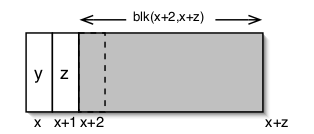
\includegraphics[scale=0.4]{node_demo.png}

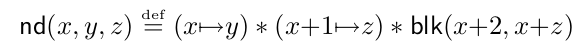
\includegraphics[scale=0.4]{node_def.png}

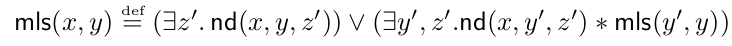
\includegraphics[scale=0.4]{mls_def.png}
\end{center}

No pointer arithmetic outside \texttt{nd}.
\end{frame}

\begin{frame}\frametitle{Abstraction: An Example}
Definition of \texttt{nd}:

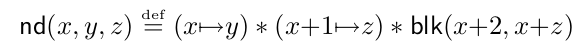
\includegraphics[scale=0.4]{node_def.png}

Example:

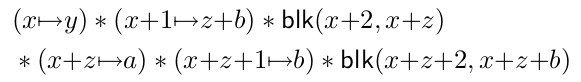
\includegraphics[scale=0.4]{example_1.png}

By the definition of \texttt{nd}:

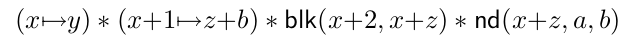
\includegraphics[scale=0.4]{example_2.png}

A true implication:

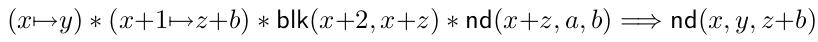
\includegraphics[scale=0.4]{example_3.png}

Difficulty: information lost.

\end{frame}

\begin{frame}\frametitle{Program Considered}
\begin{center}
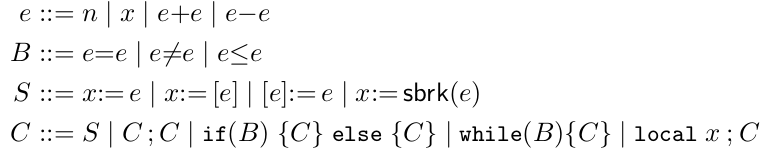
\includegraphics[scale=0.45]{program_considered.png}
\end{center}
Concrete states:

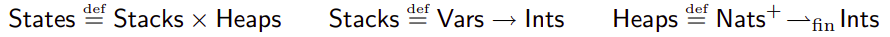
\includegraphics[scale=0.45]{states.png}


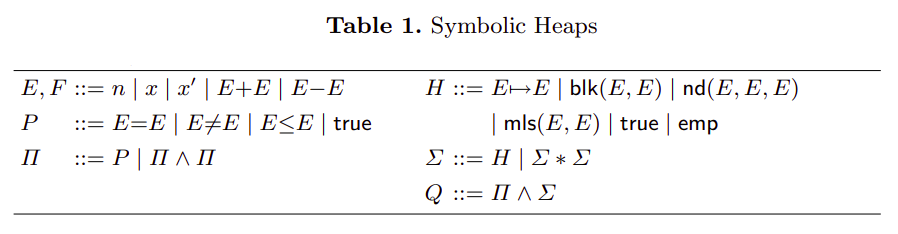
\includegraphics[scale=0.45]{sh.png}

\end{frame}

\begin{frame}\frametitle{Basic Settings}
Symbolic heap: $Q$, which contains primed variables.

Let $\mathtt{SH}$ be the set of all symbolic heap.

Abstract domain $\mathcal{D}$:

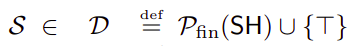
\includegraphics[scale=0.40]{abstractdomain.png}

\textbf{Concretization: }

The concretization $\gamma(Q)$ of $Q$ is the set of concrete states satisfying $\exists \vec{y'}. Q$.

The concretization of $\mathcal{S}$:
\begin{center}
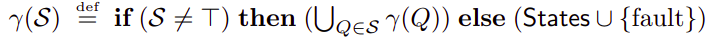
\includegraphics[scale=0.4]{concretization.png}
\end{center}

Elements in $\mathcal{D}$ are ordered by subset relation:
\begin{center}
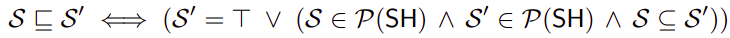
\includegraphics[scale=0.4]{order.png}
\end{center}



\end{frame}

\begin{frame}\frametitle{Abstraction Function}
The abstraction function $\mathtt{Abs}: \mathcal{D}\rightarrow\mathcal{D}$ contains five phases:
\begin{itemize}
\item Synthesize node from RAM configurations.
\item Simplify arithmetic expressions from explosion of arithmetic constraints.

\item Abstract size field.
\item Reason about multiword list.
\item Filter out inconsistent symbolic heaps.
\end{itemize}

\end{frame}

\begin{frame}\frametitle{Abstraction Rules: Node Synthesis }
\begin{center}
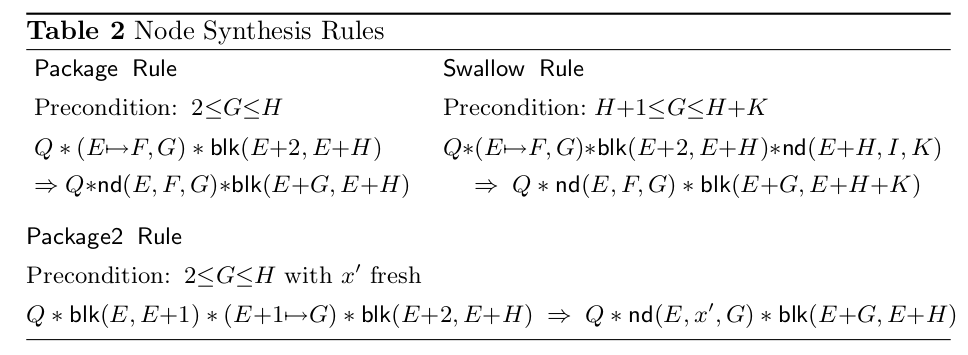
\includegraphics[scale=0.4]{nodesynthesisrule.png}

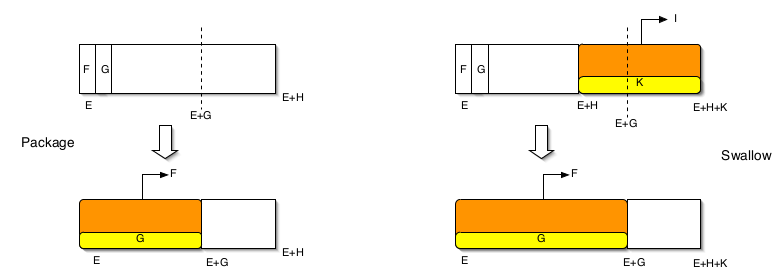
\includegraphics[scale=0.4]{nodesynthesis.png}
\end{center}
\end{frame}

\begin{frame}\frametitle{Abstraction Rules: Arithmetic Simplification}
A symbolic heap $Q\equiv \Pi \wedge \Sigma$ is in \emph{n-simple form} iff:
\begin{center}
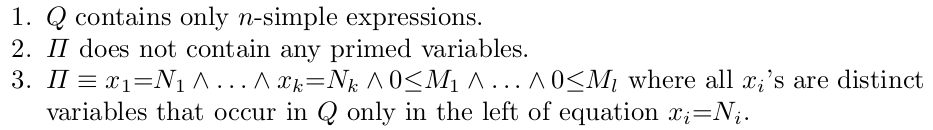
\includegraphics[scale=0.4]{n-simple.png}

\end{center}
where 
\begin{center}

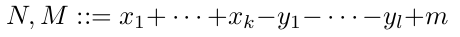
\includegraphics[scale=0.4]{mn.png}
\end{center}

\end{frame}

\begin{frame}\frametitle{Abstraction Rules: Arithmetic Simplification}
\begin{center}
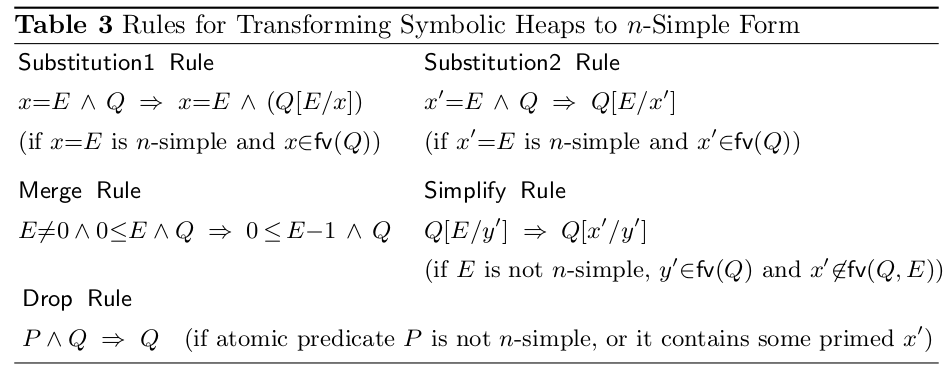
\includegraphics[scale=0.4]{arithrule.png}
\end{center}
\end{frame}

\begin{frame}\frametitle{Abstraction Rules: Abstract Size Field}
\begin{center}
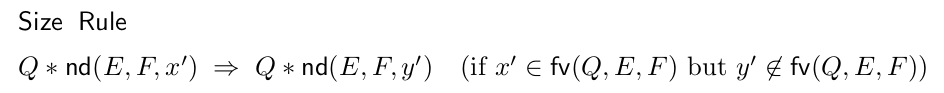
\includegraphics[scale=0.4]{size.png}
\end{center}
\end{frame}

\begin{frame}\frametitle{Abstraction Rules: Multilist Rules}
\begin{center}
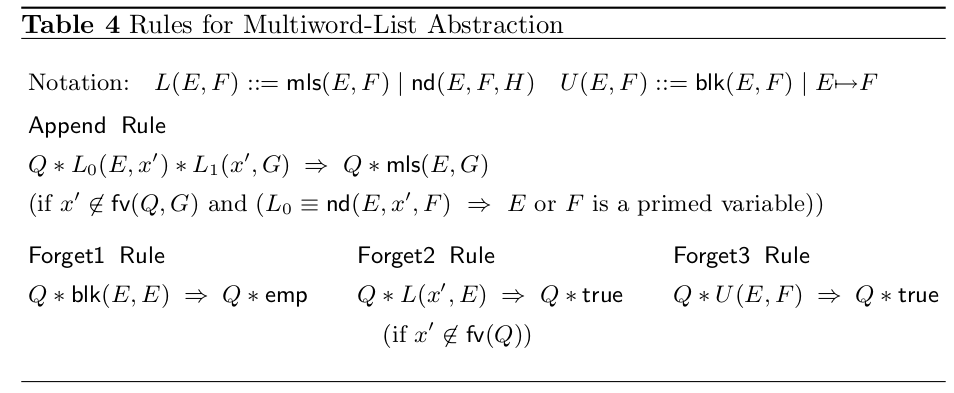
\includegraphics[scale=0.4]{mtw.png}
\end{center}
\end{frame}

\begin{frame}\frametitle{Abstraction Rules: Filter Inconsistency}
\begin{center}
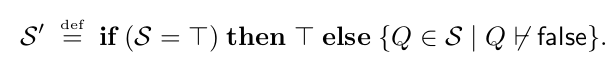
\includegraphics[scale=0.4]{inc.png}
\end{center}
\end{frame}

\begin{frame}\frametitle{$n$-Canonical  Form}
\begin{center}
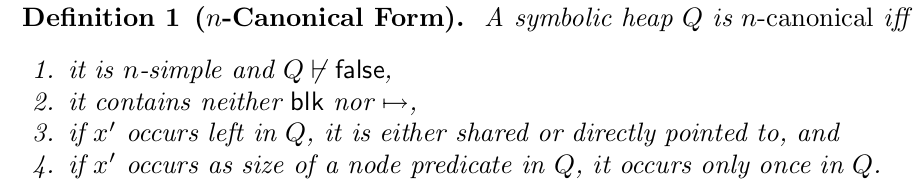
\includegraphics[scale=0.4]{ncan.png}
\end{center}
Use $\mathcal{C}_n$ as the set of $n$-canonical form in $\mathcal{D}$.


\end{frame}

\begin{frame}\frametitle{Widening Operator}
The function $\mathtt{rep}$
\begin{center}
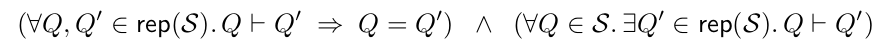
\includegraphics[scale=0.4]{rep.png}

\end{center}

and the widening operator is given by:

\begin{center}
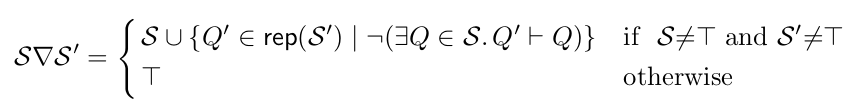
\includegraphics[scale=0.4]{widen.png}

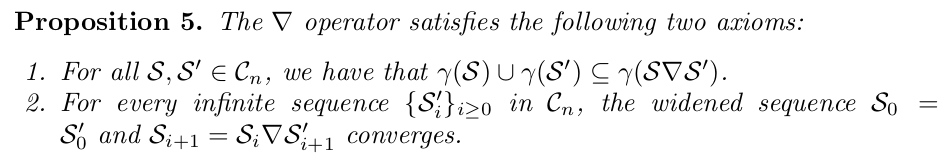
\includegraphics[scale=0.4]{axiom.png}
\end{center}

\end{frame}

\begin{frame}\frametitle{Abstract Semantic}

\begin{center}
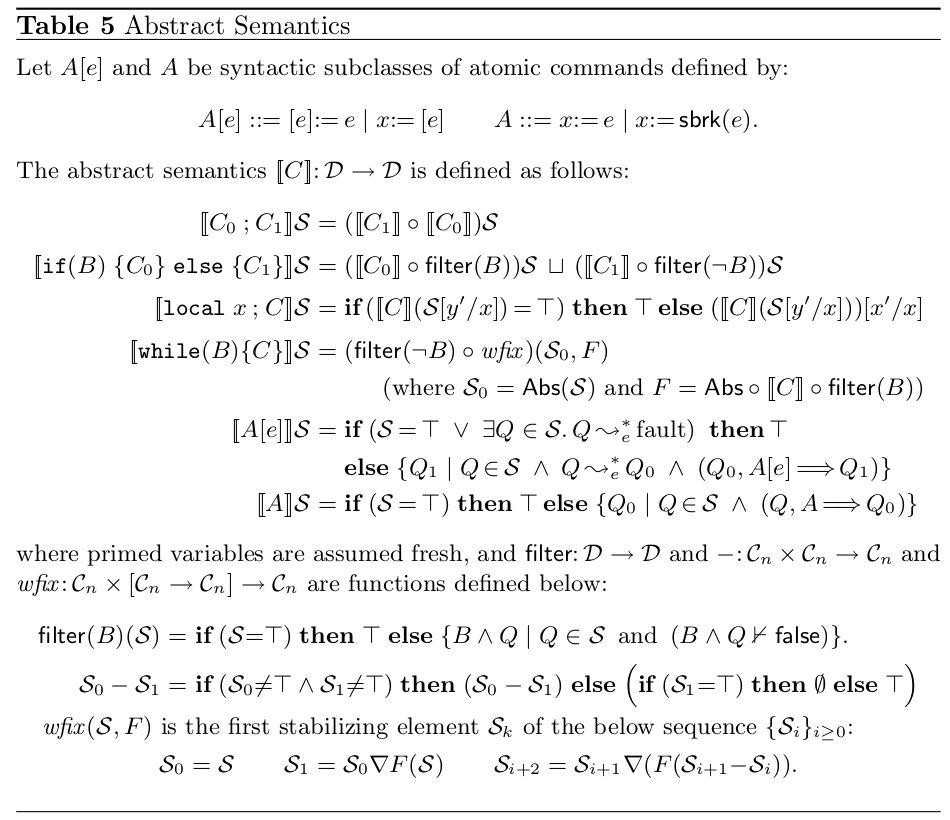
\includegraphics[scale=0.32]{table5.png}
\end{center}
\end{frame}

\begin{frame}\frametitle{Soundness}
\begin{center}
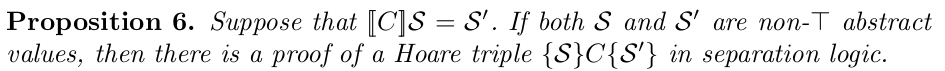
\includegraphics[scale=0.4]{sound.png}
\end{center}
\end{frame}

\end{document}